\usepackage{amsmath}
\usepackage{amssymb}
\chapter{Klassische Skalierungsmethoden}

\section{Pixel-Verdopplung}
Die Pixel-Verdopplung vergrößert das Bild indem jeder Pixel dupliziert wird.
Diese Methode kann schnell und einfach umgesetzt werden, indem jeder Pixelwert einfach auf den Nachbarpixel übertragen wird. 
Wenn Bilder mit dieser Methode stark vergrößert werden, ergeben sich oft pixelige und unscharfe Ausgaben, da die Details nicht wirklich vorhanden sind, sondern nur durch die Duplizierung von Pixeln aufgefüllt werden. 
Aus diesem Grund wird Pixel-Verdopplung oft als eine minderwertige Skalierungsmethode betrachtet und findet in professinellen Anwendungen selten Gebrauch.\footfullcite{WANG1983363}


\newpage
Eine Beispielhafte Implementierung in Python sieht folgendermaßen aus: 

\begin{figure}
    \centering
    \begin{lstlisting}
class PixelVerdopplung(Image):
    def __init__(self, path):
        extend = "p2"
        super().__init__(path, extend)
    
    def manipulate(self, new_size):
        super().manipulate(new_size)
    
        for y in range(self.new_height):
            for x in range(self.new_width):
                x_old = int(x / (self.new_width / self.width))
                y_old = int(y / (self.new_height / self.height))
    
                # Check that x_old and y_old are within
                # bounds of original image
                if x_old >= self.width:
                    x_old = self.width - 1
                if y_old >= self.height:
                    y_old = self.height - 1
    
                old_pixel = self.img.getpixel((x_old, y_old))
                self.newImg.putpixel((x, y), old_pixel)
    
        return self.save()
\end{lstlisting}
    \caption{Python-Implementierung der Klasse zu Verdopplung von Pixeln.}
    \label{fig:my_label}
\end{figure}


Die vorliegende Implementierung in Python beschreibt die Realisierung der Pixelverdopplungsklasse, welche in der Lage ist, ein größeres Bild zu erzeugen, indem die leeren Pixel mit demselben Pixelwert wie der nächste Nachbarpixel befüllt werden.

Der Code ist darauf ausgelegt, eine einfache Möglichkeit bereitzustellen, um ein Bild auf eine höhere Auflösung zu skalieren, wodurch fehlende Details ausgeglichen werden können. Dabei wird eine lineare Interpolation auf der Basis der Nachbarpixel durchgeführt, um das neue Bild zu generieren.

Die Klasse "PixelVerdopplung" erbt von der Klasse "Image" und besitzt einen Konstruktor, der den Pfad zum Bild und die Erweiterung "p2" als Argumente erhält. Die Methode "manipulate" ist dafür zuständig, das Bild auf die gewünschte Größe zu skalieren und zu manipulieren.

Innerhalb der Methode werden Schleifen durchlaufen, um jeden neuen Pixel im manipulierten Bild zu generieren. Die Koordinaten des jeweiligen alten Pixels werden durch Division der neuen Koordinaten durch die Skalierungsfaktoren berechnet und auf den nächstgelegenen Integer gerundet.

Um sicherzustellen, dass die berechneten Koordinaten innerhalb der Grenzen des ursprünglichen Bildes liegen, werden sie in einem nächsten Schritt auf den maximalen Index des Bildes zurückgesetzt, falls sie außerhalb liegen sollten. Anschließend wird der Pixelwert des entsprechenden alten Pixels abgerufen und als neuer Pixel an der berechneten Stelle im neuen Bild platziert.

Die Implementierung dieses Algorithmus stellt eine einfache Möglichkeit dar, um ein Bild auf eine höhere Auflösung zu skalieren, wodurch ein besseres visuelles Ergebnis erzielt werden kann. Dabei ist darauf zu achten, dass die lineare Interpolation eine höhere Laufzeit und Speicheranforderungen aufweist als andere Interpolationsmethoden.



\section{Nearest-Neighbor-Interpolation}
Die Nearest-Neighbor-Interpolation ist eine weitere Methode zur Skalierung von Bildern. 
Es wird für jeden Pixel im Ausgabebild der am nächsten liegende Pixel im Eingabebild ausgewählt und der Farbwert des ausgewählten Pixels wird als Farbwert des entsprechenden Pixels im Ausgabebild verwendet.
Die Verwendung von Nearest-Neighbor-Interpolation ist einfach und schnell zu implementieren. 
Aufgrund ihrer geringen Komplexität ist sie daher sehr beliebt. 
Die Methode eignet sich besonders gut für die Vergrößerung von Bildern mit großen, einheitlichen Bereichen oder harten Kanten. 


Bei der Verkleinerung von Bildern erleiden diese jedoch oft einen Qualitätsverlust.
Hier kommt es zu Unschärfe und Blockbildung. 
Diese Effekt verstärkt sich, wenn das Verhältniss zwischen Quellbild und Audgabebild kein Vielfaches ist. 
\begin{acronym}
  \acro{NNI}{Nearest Neighbor Interpolation}
\end{acronym}
\begin{lstlisting}
import numpy as np
import cv2

def nearest_neighbor_interpolation(image, scale_factor):
    new_size = (int(image.shape[1] * scale_factor), int(image.shape[0] * scale_factor))
    
    scaled_image = np.zeros(new_size + (image.shape[2],), dtype=np.uint8)
    for i in range(new_size[0]):
        for j in range(new_size[1]):
            x = int(i / scale_factor)
            y = int(j / scale_factor)
            scaled_image[j, i] = image[y, x]
    
    return scaled_image


image = cv2.imread('example_image.jpg')
scaled_image = nearest_neighbor_interpolation(image, 2)
cv2.imshow(image)
cv2.imshow(scaled_image)
\end{lstlisting}\footfullcite{jiang2015quantum}
%TODO @Marc kannst du mir ne Schöne Grafik machen, wo du diesen Code kurz über unser Beispielbild laufen lässt und wir so nen rechts/links Vergleich haben? 
\section{Bilineare Interpolation}

Interpolation cool weil, schnell und ergebniss recht schön.
%TODO Noch was schreiben


\begin{figure}
    \centering
    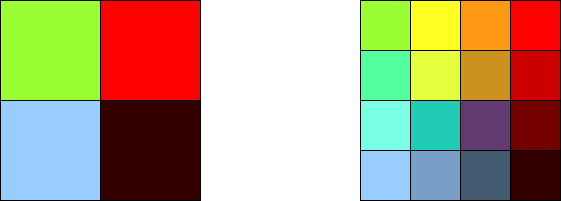
\includegraphics[width=\textwidth]{img/pixel_verdopplung.png}
    \caption{Beispielgrafik zur Pixelverdopplung.}
    \label{fig:my_label}
\end{figure}

\begin{figure}
    \centering
    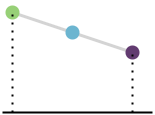
\includegraphics{img/pixel_verdopplung_graph.png}
    \caption{Graph über bilineare Skalierung.}
    \label{fig:my_label}
\end{figure}


\begin{lstlisting}
for y in range(self.new_height):
    for x in range(self.new_width):
        x_old = x / (self.new_width / self.width)
        y_old = y / (self.new_height / self.height)

        # Find the surrounding pixels
        x1 = int(x_old)
        x2 = min(x1 + 1, self.width - 1)
        y1 = int(y_old)
        y2 = min(y1 + 1, self.height - 1)

        # Check if x2 and y2 are out of bounds, if they are substract one
        if x2 == self.width - 1:
            x2 = x1
            x1 -= 1
        if y2 == self.height - 1:
            y2 = y1
            y1 -= 1

        # Find the weights
        w1 = (x2 - x_old) * (y2 - y_old)
        w2 = (x_old - x1) * (y2 - y_old)
        w3 = (x2 - x_old) * (y_old - y1)
        w4 = (x_old - x1) * (y_old - y1)

        # Get the pixel values of the surrounding pixels
        p1 = self.img.getpixel((x1, y1))
        p2 = self.img.getpixel((x2, y1))
        p3 = self.img.getpixel((x1, y2))
        p4 = self.img.getpixel((x2, y2))

        # Interpolate the pixel value
        new_pixel = (
            int(w1 * p1[0] + w2 * p2[0] + w3 * p3[0] + w4 * p4[0]),
            int(w1 * p1[1] + w2 * p2[1] + w3 * p3[1] + w4 * p4[1]),
            int(w1 * p1[2] + w2 * p2[2] + w3 * p3[2] + w4 * p4[2])
        )
        self.newImg.putpixel((x, y), new_pixel)
\end{lstlisting}\footfullcite{1409828}

\section{Bicubische Interpolation}

\subsection{Mathematische Grundlagen}

Die bikubische Interpolation ist ein mathematisches Verfahren zur Schätzung der Werte einer kontinuierlichen Funktion an einer gegebenen Stelle, indem eine Funktion mit kubischen Polynomen verwendet wird, die durch benachbarte Funktionswerte verläuft. Dabei wird das umliegende Gebiet untersucht und die Werte werden basierend auf der Stichprobentheorie geschätzt.

Die bikubische Interpolationsformel ist eine Erweiterung der Bilinearinterpolation auf vier umliegende Pixel und verwendet eine Funktion, die durch benachbarte Funktionswerte verläuft. Die resultierende Funktion ist stetig differenzierbar und besitzt glatte partielle Ableitungen.

Im Vergleich zu anderen Interpolationsverfahren wie der bilinearen Interpolation und der Lanczos-Interpolation hat die bikubische Interpolation den Vorteil, dass sie eine höhere Genauigkeit bei der Schätzung von Pixelwerten bietet. Ein Nachteil ist jedoch, dass sie im Allgemeinen höhere Rechenaufwendungen erfordert.

Die Fourier-Analyse und die Fourier-Transformationen spielen eine wichtige Rolle bei der Bildinterpolation, da sie es ermöglichen, die Funktion in den Frequenzraum zu transformieren und damit eine effektivere Interpolation zu erreichen.

\subsection{Algorithmische Implementierung}

Die bikubische Interpolation erfolgt durch die Auswahl von umgebenden Pixeln und deren Gewichte sowie der Berechnung der neuen Pixelwerte. Eine Möglichkeit zur Optimierung der Leistung besteht darin, Lookup-Tabellen vorzubereiten, Parallelisierungstechniken zu verwenden und die Speicherverwaltung zu optimieren.

Grenzfälle und Randbedingungen können bei der bikubischen Interpolation auftreten und müssen effektiv behandelt werden. Die algorithmische Implementierung der bikubischen Interpolation kann mit anderen Interpolationsverfahren wie der bilinearen Interpolation und der Lanczos-Interpolation verglichen werden.

Ein Beispiel für die Implementierung der bikubischen Interpolation in Python ist der folgende Code:

Die Methode `manipulate` der Klasse `BicubicInterpolation` implementiert die bicubische Interpolation für das Vergrößern von Bildern. Der wichtigste Teil des Codes ist die Schleife, die über jedes Pixel einen Kernel berechnet, der die jeweiligen Gewichte der benachbarten Pixel erechnet. In den genannten Zeilen wird ein 4x4-Kern um das aktuelle Pixel herum gebildet und für jeden Pixel im Kern werden die Gewichte berechnet. Dabei wird die `_get_weight`-Funktion aufgerufen, welche auf der Basis einer kubischen Kurve das Gewicht für einen bestimmten Abstand berechnet. Die berechneten Gewichte werden in eine Liste `weights` hinzugefügt. Diese Gewichte dienen später bei der Interpolation des aktuellen Pixels als multiplikative Faktoren für die umliegenden Pixel im Originalbild.

\begin{lstlisting}
weights = []
for j in range(-1, 3):
    for i in range(-1, 3):
        weight = _get_weight(i - dx) * _get_weight(dy - j)
        weights.append(weight)
\end{lstlisting}

\subsection{Analyse der Leistung}

Zur Bewertung der Leistung von Bildinterpolationsverfahren werden verschiedene Kriterien verwendet, einschließlich der visuellen Qualität, der Genauigkeit und der Berechnungseffizienz. Die Leistung der bikubischen Interpolation kann mit anderen Interpolationstechniken anhand von Testbildern und Datensätzen verglichen werden. Dabei werden verschiedene Parameter wie Bildgröße, Auflösung und Inhalt untersucht, um ihre Auswirkungen auf die Leistung der bikubischen Interpolation zu analysieren. %...


% Ich hab das obere vom bot schreiben lassn







    \subsection{Mathematische Grundlagen}

    Erläuterung der mathematischen Grundlagen der bikubischen Interpolation, einschließlich der Verwendung von kubischen Polynomen und der Stichprobentheorie.
    Herleitung der bikubischen Interpolationsformel und der Eigenschaften der resultierenden Funktion.
    Diskussion der Vor- und Nachteile der Verwendung kubischer Funktionen für die Interpolation im Vergleich zu anderen Funktionstypen.
    Überblick über die Rolle der Fourier-Analyse und der Fourier-Transformationen bei der Bildinterpolation und wie sich dies auf die bikubische Interpolation bezieht.

    \subsection{Algorithmische Implementierung}

    Überblick über die algorithmischen Schritte bei der bikubischen Interpolation, einschließlich der Auswahl der umgebenden Pixel und der Gewichte sowie der Berechnung der neuen Pixelwerte.
    Diskussion von Techniken zur Optimierung der Leistung der bikubischen Interpolation, wie z. B. die Vorberechnung von Lookup-Tabellen, Parallelisierung und Speicherverwaltung.
    Untersuchung von Grenzfällen und Randbedingungen, die bei der bikubischen Interpolation auftreten können, und wie diese effektiv behandelt werden können.
    Vergleich der algorithmischen Implementierung der bikubischen Interpolation mit anderen Interpolationsverfahren, wie z.B. der bilinearen Interpolation und der Lanczos-Interpolation.

    \subsection{Implementation}
    \begin{lstlisting}
    from scipy import interpolate
    import numpy as np

    def bicubic_interpolation(image, new_shape):
    height, width = image.shape[:2]
    x = np.arange(0, width)
    y = np.arange(0, height)
    f = interpolate.interp2d(x, y, image, kind='cubic')
    new_width, new_height = new_shape
    new_x = np.linspace(0, width-1, new_width)
    new_y = np.linspace(0, height-1, new_height)
    return f(new_x, new_y)
    \end{lstlisting}
    \subsection{Analyse der Leistung}

    Erläuterung der Kriterien, die zur Bewertung der Leistung von Bildinterpolationsverfahren verwendet werden, einschließlich der visuellen Qualität, der Genauigkeit und der Berechnungseffizienz.
    Vergleich der Leistung der bikubischen Interpolation mit anderen Interpolationstechniken unter Verwendung einer Reihe von Testbildern und Datensätzen.
    Untersuchung der Auswirkungen verschiedener Parameter wie Bildgröße, Auflösung und Inhalt auf die Leistung der bikubischen Interpolation.
    Diskussion der potenziellen Einschränkungen und Kompromisse, die mit der Verwendung der bikubischen Interpolation verbunden sind, sowie der Faktoren, die ihre Leistung in verschiedenen Kontexten beeinflussen können.

    \subsection{Anwendungen}

    Überblick über die verschiedenen Anwendungen der bikubischen Interpolation in der Bildverarbeitung, einschließlich Bildskalierung und -größenänderung, Bildrotation und -transformation sowie Bildentrauschung und -wiederherstellung.
    Diskussion der spezifischen Herausforderungen und Möglichkeiten, die sich in verschiedenen Anwendungsbereichen ergeben, z. B. in der medizinischen Bildgebung, der Satellitenbildgebung und der Videoverarbeitung.
    Erforschung der potenziellen Vor- und Nachteile der bikubischen Interpolation in verschiedenen Anwendungen und der Faktoren, die ihre Eignung für bestimmte Aufgaben beeinflussen können.

    \subsection{Erweiterungen und Variationen}

    Erläuterung der verschiedenen Erweiterungen und Variationen der bikubischen Interpolation, wie z. B. Super-Resolution-Techniken, Multiskalen- und pyramidenbasierte Interpolation und adaptive Interpolationstechniken.
    Diskussion der Vor- und Nachteile dieser Varianten und ihrer Eignung für verschiedene Bildtypen und Anwendungen.
    Erkundung potenzieller künftiger Forschungsrichtungen in diesem Bereich, z. B. auf Deep Learning basierende Ansätze, ungleichmäßige und unregelmäßige Abtastverfahren sowie mehrdimensionale und mehrkanalige Interpolation.


\section{Lanczos-Interpolation}
Die Lanczos-Interpolation ist eine Methode zur Rekonstruktion von Werten im Bild aus diskreten Abtastungen. 
In diesem Abschnitt wird die mathematische Grundlage und die praktische Anwendung der Lanczos-Interpolation kurz erläutert.

\subsection{Mathematische Grundlage}

Die Lanczos-Interpolation basiert auf der Idee, ein kontinuierliches Signal $f(x)$ durch eine Summe von gewichteten Basisfunktionen zu approximieren. 
Dieses Signal können zum Beispiel Farbwerte in einem Bild sein.
Die Basisfunktionen werden durch das sogenannte Lanczos-Kernel definiert:

\begin{equation}
MARC HIER Formel aus BILD EINFÜGEN
\end{equation}
\footfullcite{duchon1979lanczos}

Das Lanczos-Kernel hat eine kompakte Trägerfunktion.
Eine kompakte Träägerformel bedeutet, sie ist nur in einem begrenzten Bereich von Null verschieden. 
In der Praxis hat dies den Vorteil, dass das Signalrauschen in Bereichen außerhalb des Bereichs im Signalraum reduziert wird und somit eine bessere Interpolation des Signals erreicht werden kann.
Die Gewichtungen der Basisfunktionen werden durch die Interpolationskoeffizienten bestimmt, die durch die diskreten Abtastungen des Signals berechnet werden.

Die Lanczos-Interpolation wird in der Regel auf gleichmäßig verteilten Stützstellen angewendet. 
Die Interpolationsmethode verwendet diese Stützstellen als Ausgangspunkt, um eine Schätzung des Signals an anderen Orten zu berechnen. 
Seien $x_1, x_2, \ldots, x_n$ die Stützstellen des Signals und $y_1, y_2, \ldots, y_n$ die zugehörigen Abtastungen. Die Interpolationsfunktion $s(x)$ kann dann wie folgt berechnet werden:

\begin{equation}
Interpolationsfunktion bro hilfe @marc
\end{equation}

wobei $h$ der Abstand zwischen den Stützstellen ist.
\footfullcite{BENTBIB2016233}

\subsection{Praktische Anwendung}

Die Lanczos-Interpolation findet Anwendung in vielen Bereichen der Bildverarbeitung. 
Ein Anwendungsbeispiel ist die Upsampling von digitalen Bildern, um eine höhere Auflösung zu erreichen.

Die praktische Umsetzung der Lanczos-Interpolation erfordert die Berechnung der Interpolationskoeffizienten und die Bestimmung der Stützstellen des Signals. 
In der Regel werden hierfür spezielle Algorithmen eingesetzt, die auf der effizienten Berechnung der Basisfunktionen basieren.

\\Hier Implementierung einfügen (TODO) 

\section{Zusammenfassung zu Vor- und Nachteilen von Techniken in der Bildverarbeitung}

In der Bildverarbeitung gibt es verschiedene Techniken, die verwendet werden können, um ein Bild zu bearbeiten oder zu manipulieren. 
In diesem Abschnitt werden wir uns mit einigen gängigen Techniken zur Interpolation von Bildern beschäftigen, nämlich Pixelverdopplung, Nearest Neighbour Interpolation, Bilineare Interpolation, Bicubische Interpolation und Lanczos Interpolation. 
Wir werden jeweils auf die Vor- und Nachteile dieser Techniken eingehen.

\subsection{Pixelverdopplung}

Bei der Pixelverdopplung wird jedes Pixel im Bild einfach dupliziert, um ein größeres Bild zu erzeugen. 
Diese Methode ist einfach und schnell, aber sie führt oft zu einer Verzerrung des Bildes und kann zu einer verschlechterten Bildqualität führen.

\subsection{Nearest Neighbour Interpolation}

Die Nearest Neighbour Interpolation ist eine einfache Interpolationsmethode, bei der jeder neue Pixelwert durch den nächstgelegenen Pixelwert im Originalbild bestimmt wird. 
Diese Methode ist einfach und schnell, aber sie führt oft zu einem "Treppeneffekt" im Bild, da die Pixelwerte nicht kontinuierlich interpoliert werden.

\subsection{Bilineare Interpolation}

Die bilineare Interpolation ist eine Methode, bei der die neuen Pixelwerte aus einer bilinearen Funktion berechnet werden, die aus den vier nächstgelegenen Pixeln im Originalbild abgeleitet wird. 
Diese Methode führt oft zu einer glatteren Interpolation als die Nearest Neighbour Interpolation, aber es kann immer noch zu einem "Verwischen" des Bildes kommen.

\subsection{Bicubische Interpolation}

Die bicubische Interpolation ist eine Methode, bei der die neuen Pixelwerte aus einer bicubischen Funktion berechnet werden, die aus den sechzehn nächstgelegenen Pixeln im Originalbild abgeleitet wird.
Diese Methode führt oft zu einer noch glatteren Interpolation als die bilineare Interpolation, aber sie kann auch zu einer Überbetonung von Bildstrukturen führen.

\subsection{Lanczos Interpolation}
y
Die Lanczos Interpolation ist eine Methode, bei der die neuen Pixelwerte aus einer Lanczos-Funktion berechnet werden, die aus einer begrenzten Anzahl von nächstgelegenen Pixeln im Originalbild abgeleitet wird. 
Diese Methode führt oft zu einer sehr glatten Interpolation und reduziert das Rauschen im Bild, aber sie kann auch zu einer gewissen Unschärfe im Bild führen.

\subsection{Vergleich und Zusammenfassung}

Insgesamt gibt es keine "beste" Methode zur Interpolation von Bildern, da jede Methode ihre eigenen Vor- und Nachteile hat. 
Die Wahl der Methode hängt von den spezifischen Anforderungen und Einschränkungen ab, die für die jeweilige Anwendung gelten. 
Die Wahl einer geeigneten Interpolationsmethode kann jedoch die Bildqualität erheblich verbessern und zu einer effektiveren Bildverarbeitung führen.
\newpage